\chapter{Proof-of-Concept Applicatie}
\label{ch:ontwikkeling}

\section{Inleiding}

Dit hoofdstuk dient als een uitgebreide toelichting op de softwareoplossing die binnen deze bachelorproef is ontwikkeld.
Eerst zullen de verschillende componenten van de applicatie worden besproken, gevolgd door een gedetailleerde uitleg hoe de applicatie kan worden gebruikt.
Aangezien er rekening gehouden werd met het effectief inzetten van de applicatie in de praktijk, zullen ook de gebruikte technologieën en technische keuzes worden toegelicht.
Zo kan de software bij opeenvolgende bachelorproeven iteratief verder ontwikkeld worden voor nieuwe toepassingen en verbeteringen.

\section{Applicatiecomponenten en Gebruikersinteractie}

De workflow die bedacht werd voor de proof-of-concept applicatie, om van ruwe data naar bruikbare metrieken te gaan, kan als volgt worden samengevat:
\begin{enumerate}
    \item Er worden één of meerdere `kalibratie-opnames' gemaakt met de eyetrackingbril, waarbij elk object dat onderdeel is van het onderzoek, vanuit verschillende hoeken wordt gefilmd.
    \item Ook worden er evaluatieopnames gemaakt van studenten die de simulatieomgeving gebruiken, waarbij de eyetracker op het hoofd van de student wordt geplaatst.
    \item De opnames worden geïmporteerd in de applicatie via de WiFi-verbinding van de eyetrackingbril.
    \item Men geeft een naam aan de simulatieomgeving (bijvoorbeeld `Zorglab Zorgkamer') binnen de applicatie en defininieert de objecten.
    \item Daarna kan men beginnen met het labelen van de objecten in de kalibratie-opnames via de ingebouwde labeling-tool. De labeling-data dienen als basis voor het trainen of initialiseren van de analysemodellen.
    \item De applicatie is nu in staat de eyetracking-opnames van de studenten te analyseren en de metrieken te visualiseren. 
    Het visualisatiegedeelte viel buiten scope voor deze bachelorproef.
\end{enumerate}
De applicatie is dus opgebouwd uit verschillende componenten die samen een stapsgewijs proces vormen. Deze zullen hieronder verder worden toegelicht.

\subsection{Opnames Maken}

Alvorens de applicatie ontwikkeld kon worden, waren er eerst een aantal video-opnames nodig. 
In deze fase werd de Tobii eyetracking-bril van het Zorglab ontleend om vertrouwd te raken met het maken van opnames. 
Deze opnames werden thuis uitgevoerd en dienden zowel als basis voor de applicatie zelf als voor initiële experimenten met de computer vision-modellen die later zouden worden ingezet in de labeling-tool en de analyses.
Om een opname te maken hebben we twee zaken nodig: de eyetracker zelf met bijbehorende accessoires, en een laptop of computer waarop de `Tobii Pro Glasses 3 Controller'\footnote{\url{https://www.tobii.com/products/eye-trackers/wearables/tobii-pro-glasses-3/controller-app}} app is geïnstalleerd.

\begin{figure}[H]
  \centering
  
\includegraphics[width=0.6\textwidth]{placeholder.jpeg}
  \caption[]{\label{fig:todo} TODO: Foto met de benodigdheden: eyetracker, hub, laptop met app zichtbaar (eyetracker niet geconnecteerd), batterijlader, kalibratiekaart
 }
\end{figure}
% TODO: Foto met de benodigdheden: eyetracker, hub, laptop met app zichtbaar (eyetracker niet geconnecteerd), batterijlader, kalibratiekaart

De eyetracker zelf bestaat uit een hub die stroom levert aan de bril en de opnames opslaat op een SD-kaart. 
Deze hub is verbonden met de bril zelf via een ingebouwde HDMI-kabel.
De hub heeft een batterij die opgeladen kan worden met de bijgeleverde oplader. 
Eenmaal de hub ingeschakeld is, verschijnt er een WiFi-verbinding op de laptop of computer.
Deze verbinding start met `TG', gevolgd door het serienummer van de bril. Het wachtwoord voor de verbinding is `TobiiGlasses'. 
Open de Tobii Pro Glasses 3 Controller-app en observeer of het camerabeeld van de bril zichtbaar is in de app.

\begin{figure}[H]
  \centering
  
\includegraphics[width=0.6\textwidth]{placeholder.jpeg}
  \caption[]{\label{fig:todo} TODO: Foto van de app met camerabeeld zichtbaar, en de knoppen om opnames te maken
 }
\end{figure}
% TODO: Foto van de app met camerabeeld zichtbaar, en de knoppen om opnames te maken

Na het invoegen van de naam van de opname (of participant), drukt men op de knop `Record' om de opname te starten.
Voordat de opname kan starten, zal de app vragen om de bril te kalibreren. 
Dit kan gedaan worden met de bijgeleverde kalibratiekaart, die op armlengte afstand van de bril dient gehouden te worden.
Aan de participant wordt gevraagd om naar de centrale stip op de kaart te kijken, en vervolgens wordt er op de knop `Calibrate' gedrukt.
De app begint nu met het opnemen van de video, en de participant kan nu vrij rondlopen in de simulatieomgeving.

% TODO: Best-practices toevoegen?

\subsection{Importeren van Eyetracking-Opnames}

Zoals eerder vermeld heeft de Tobii eyetracker twee componenten: de bril zelf en een `hub' die stroom levert aan de bril en de opnames opslaat op een SD-kaart.
Het zou dus mogelijk zijn om de opnames via de SD-kaart te importeren, maar dit is niet praktisch aangezien de SD-kaart steeds uit de hub gehaald dient te worden.
Daarom biedt de hub ook een WiFi-verbinding aan, zodat de opnames via een netwerkverbinding kunnen worden geïmporteerd. 

Wanneer men de applicatie opent op de pagina `Browse Recordings' via de navigatiekolom, worden er twee tabellen getoond (zie figuur \ref{fig:browse-recordings})

\begin{figure}[H]
  \centering
  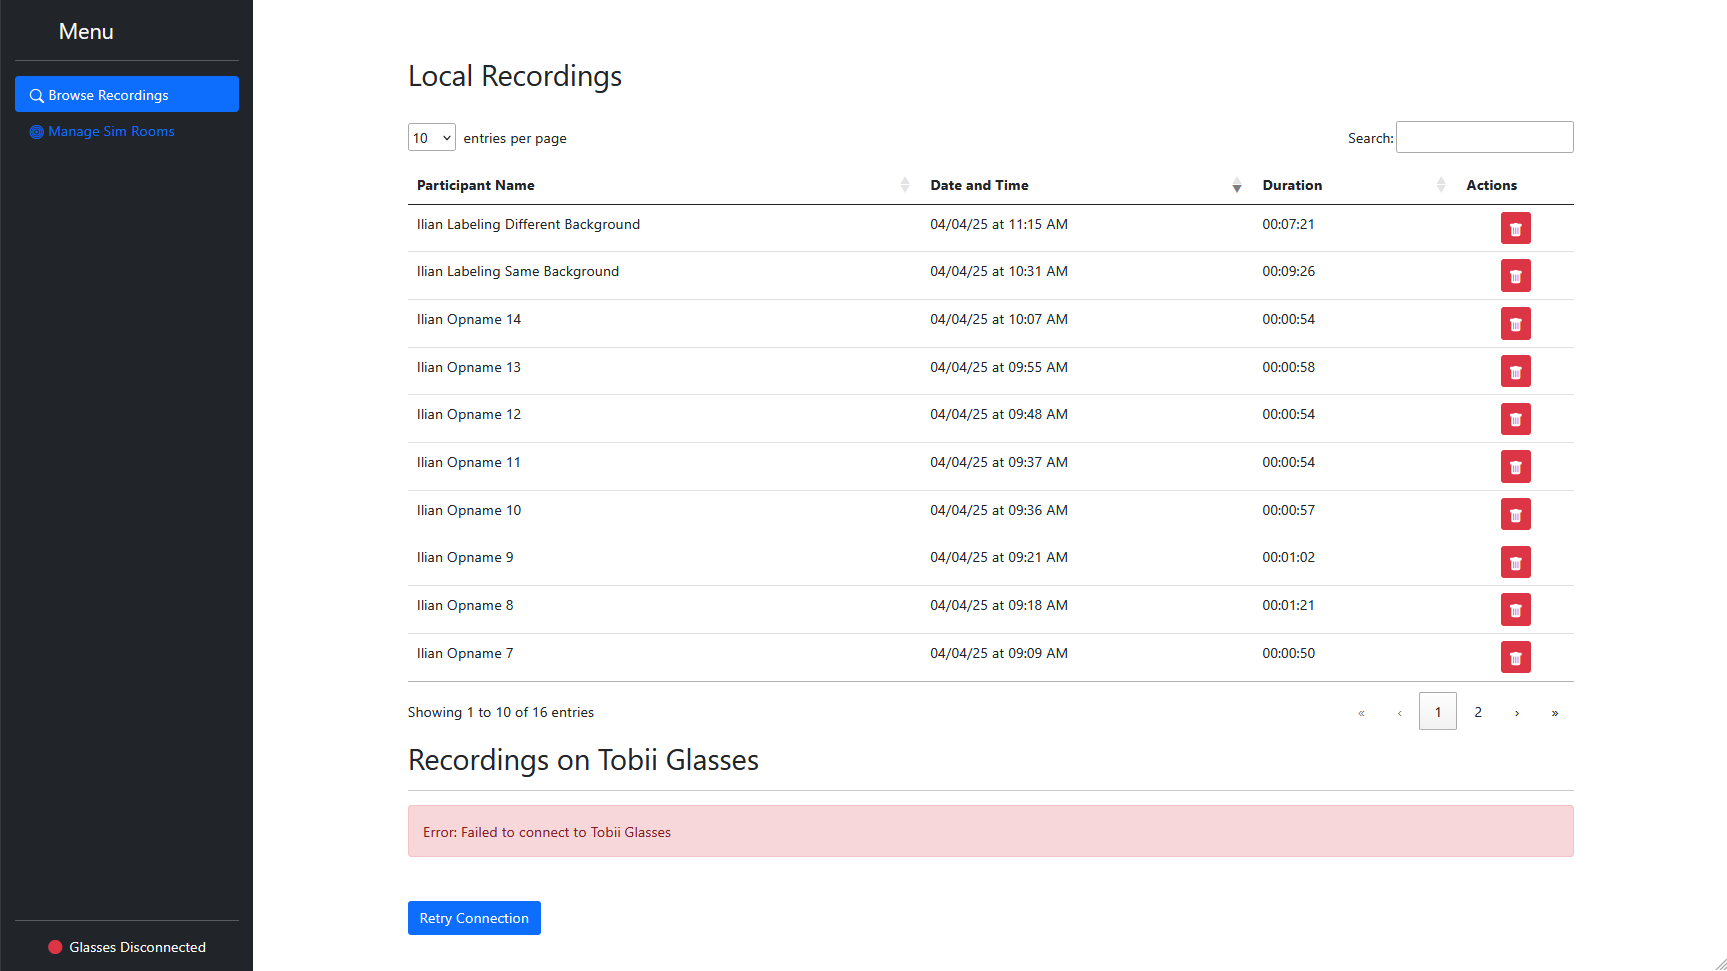
\includegraphics[width=1\textwidth]{browse-recordings.png}
  \caption[]{\label{fig:browse-recordings} Screenshot van de `Browse Recordings'-pagina waar opnames kunnen worden geïmporteerd. Hier is de bril niet verbonden met de computer. }
\end{figure}


De eerste tabel `Local Recordings' toont de opnames die lokaal zijn opgeslagen op de computer, en de onderste tabel `Recordings on Tobii Glasses' toont de opnames die zijn opgeslagen op de hub.
Indien een tabel geen opnames bevat, wordt er een passend bericht getoond.
De opnames worden getoond in tabellen met de naam van elke opname, de datum en tijd waarop deze werd gemaakt, evenals de duur van de opname. 
Het is mogelijk om opnames te verwijderen uit de `Local Recordings'-tabel door op de rode knop met het prullenbakje te klikken naast een opname. Dit heeft geen invloed op de opnames die zijn opgeslagen op de hub.
Ook kan men zoeken naar opnames via de zoekbalk bovenaan de tabellen, en kan men deze sorteren op naam, datum of duur door op de bijbehorende kolomkop te klikken.

Wanneer de bril niet verbonden is met de computer, wordt er een aangepaste melding getoond, met een knop om opnieuw te verbinden. Figuur \ref{fig:browse-recordings} toont een voorbeeld van de interface van de applicatie, waar de bril niet verbonden is met de computer.
Linksonder in de interface toont de applicatie de huidige status van de verbinding met de bril, inclusief de batterijstatus. Bij figuur \ref{fig:browse-recordings-connected} is de bril wel verbonden met de computer. 
Elke rij in de onderste tabel bevat een blauwe knop met een pijl naar beneden, waarmee een opname kan worden geïmporteerd vanuit de bril naar de computer. Dit kan enige tijd duren, afhankelijk van de grootte van de opname.

\begin{figure}[H]
  \centering
  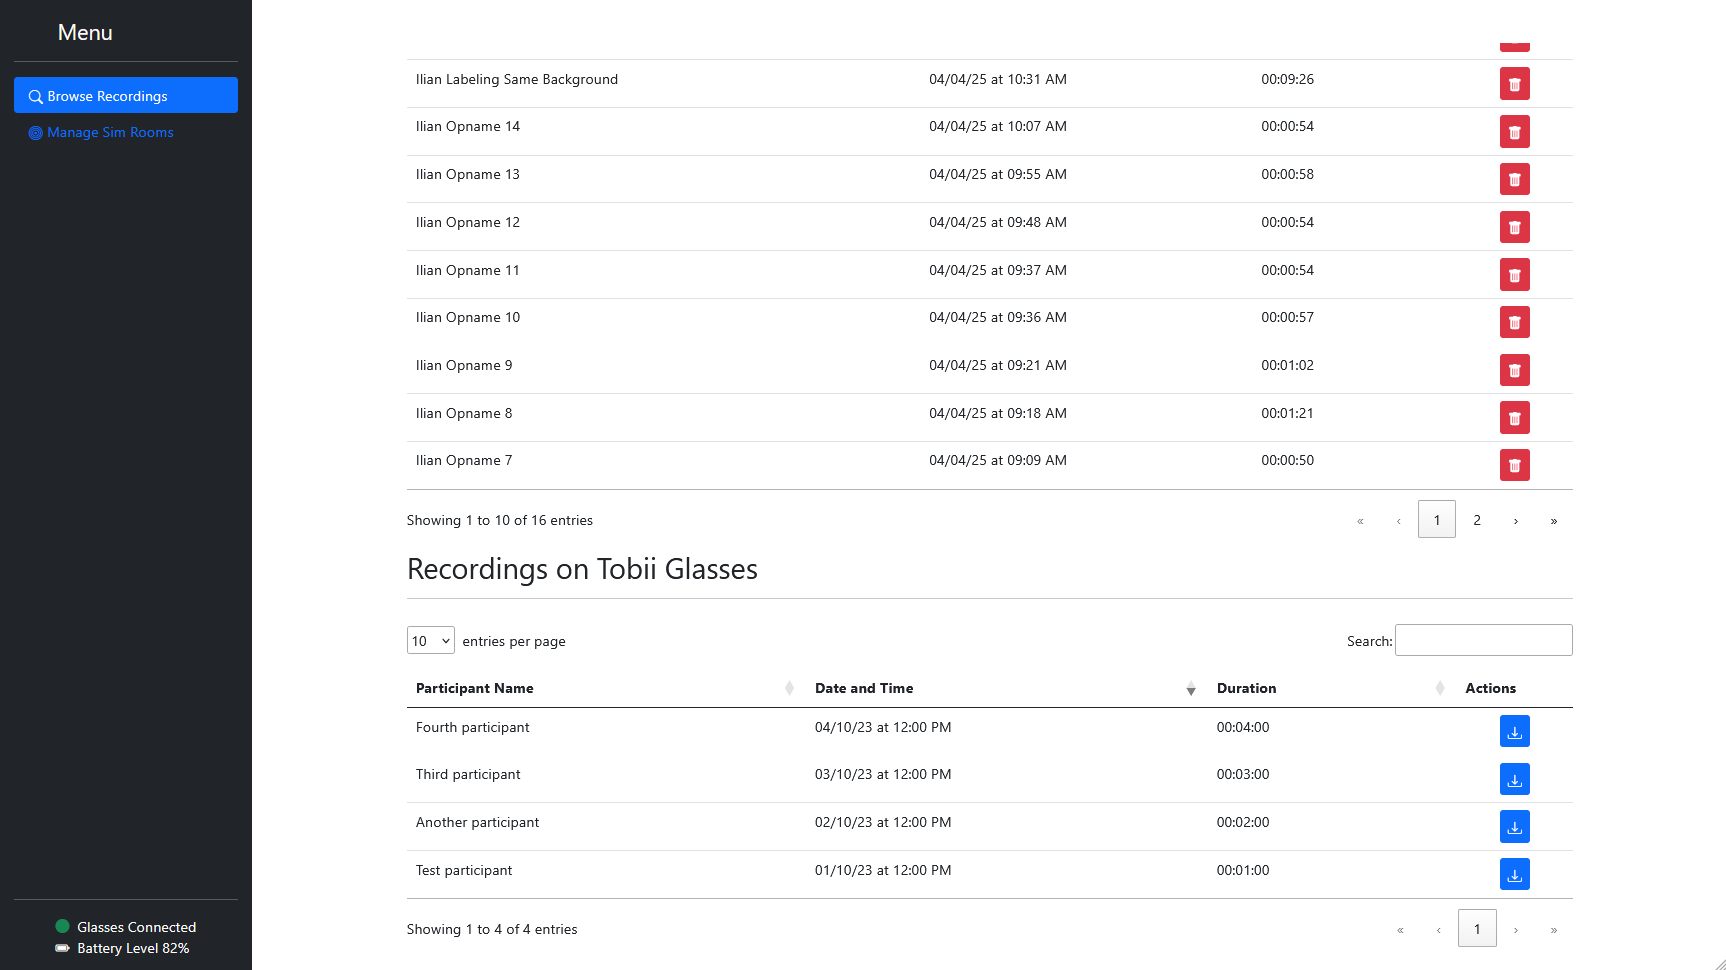
\includegraphics[width=1\textwidth]{browse-recordings-connected.png}
  \caption[]{\label{fig:browse-recordings-connected} Bij dit voorbeeld is de bril wel verbonden met de computer. Men ziet linksonder de batterijstatus van de bril. In de onderste tabel is het mogelijk om opnames te importeren vanuit de bril naar de computer. }
\end{figure}

\subsection{Simulatieruimten en Objecten}

Eens de opnames zijn geïmporteerd, kunnen we overgaan tot het definiëren van de objecten in de kalibratie-opnames. Één van de design-keuzes was om met zogenaamde `simulatieruimten` te werken die verschillende omgevingen voorstellen, elk met hun eigen objecten.
Men kan zich dus voorstellen dat men niet enkel in het Zorglab werkt, maar bijvoorbeeld ook in een echt ziekenhuis of een woonzorgcentrum. Het doel was dus om de applicatie zo gebruiksvriendelijk mogelijk te maken, om het werk van de trainers te vereenvoudigen.

\begin{figure}[H]
  \centering
  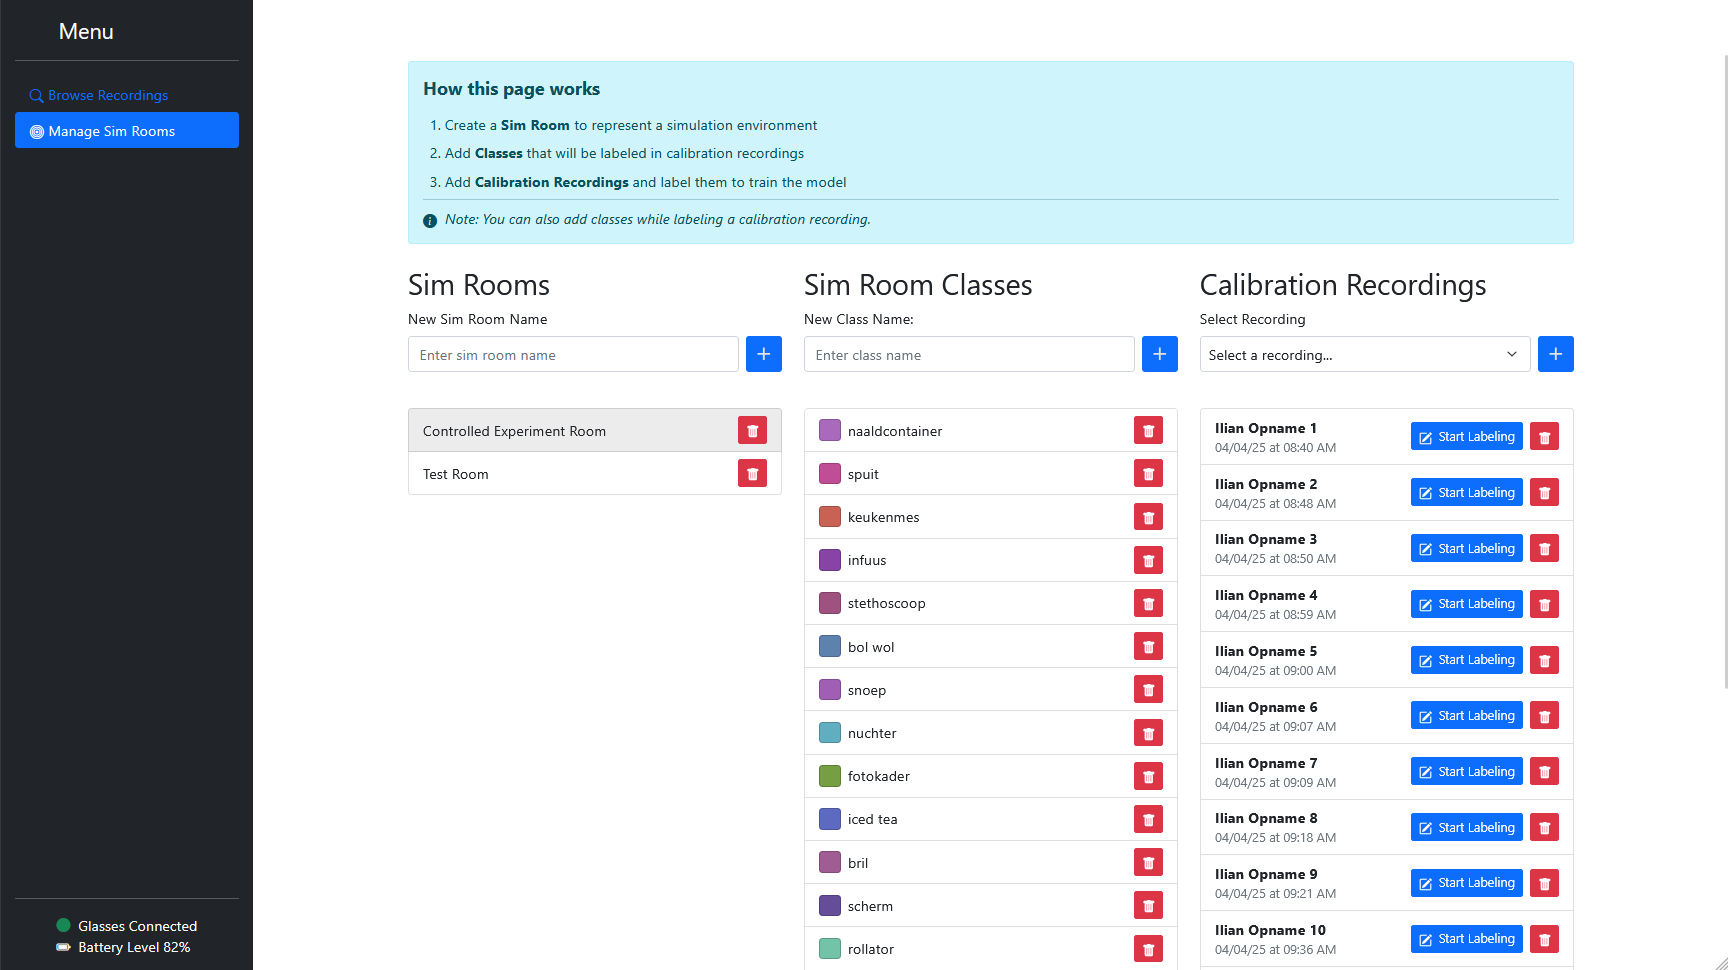
\includegraphics[width=1\textwidth]{simrooms.png}
  \caption[]{\label{fig:simrooms} Voorbeeld van de `Manage Sim Rooms'-pagina waar de simulatieomgevingen kunnen worden gedefinieerd. Hier is de `Controlled Experiment Room' geselecteerd, met een aantal objecten en kalibratie-opnames. }
\end{figure}

In figuur \ref{fig:simrooms} is een voorbeeld te zien van de pagina waar simulatieomgevingen kunnen worden gedefinieerd. 
Deze pagina heeft drie kolommen:
\begin{itemize}
    \item De eerste kolom toont de reeds gedefinieërde simulatieomgevingen, met hun naam, een knop om deze te verwijderen, en een invoerveld om meer simulatieomgevingen toe te voegen.
    \item Wanneer een simulatieomgeving is geselecteerd, worden de bijbehorende objecten getoond in de tweede kolom. Elk object krijgt automatisch een kleur toegewezen die ook gebruikt zal worden in de labeling-tool en eventueel de visualisatie van de metrieken.
    \item In de derde kolom kan men geïmporteerde opnames selecteren om deze te gebruiken als kalibratie-opnames. Elke kalibratie-opname heeft een knop `Start Labeling'. Wanneer men hierop klikt, wordt de labeling-tool geopend met de geselecteerde opname.
\end{itemize}

Merk op dat het mogelijk is om om het even welke opname te selecteren als kalibratie-opname, waardoor ook evaluatieopnames kunnen worden gebruikt!
Zo kunnen we reeds gemaakte opnames van studenten ook gebruiken om de analysemodellen te trainen.
Dit maakt het mogelijk om de opnames te analyseren op basis van manuele labels door de trainers.
Deze aanpak zal meer tijd vergen, maar is veel nauwkeuriger dan een automatische analyse. Aangezien het in deze bachelorproef gaat om geautomatiseerde analyse, werd deze optie niet verder uitgewerkt.

Wanneer men een kalibratie-opname verwijdert, heeft dit geen invloed op de opname zelf, maar enkel op de associatie met de simulatieomgeving.
Indien er in de opname werd gelabeld binnen deze simulatieomgeving, worden deze labels wel verwijderd. 
Hetzelfde geldt voor de objecten: indien een object wordt verwijderd, worden ook de labels die gemaakt werden met dit object in alle kalibratie-opnames verwijderd.

\subsection{Labeling Tool}

We hebben het al eerder gehad over de labeling-tool, maar hoe werkt deze nu precies? Dit is één van de belangrijkste onderdelen van de applicatie, en ook het meest complexe.
De labeler kunnen we openen door op de knop `Start Labeling' te klikken van een kalibratie-opname binnen de `Manage Sim Rooms'-pagina.
Bij het laden van de labeler worden alle individuele frames uit de opname gehaald en in een map opgeslagen, waardoor het enige tijd kan duren voor de tool opent. De specifieke implementatieredenen hiervoor komen later aan bod.
Het doel van de labeler is om een masker en een `bounding box' te verkrijgen binnen elke frame van de opname waarin een object zich bevindt.
Natuurlijk zou dit een grote tijdsinvestering vragen bij een volledig manuele tool: aangezien de framerate van de eyetracker 25fps (Frames per Second) is, zou dit betekenen dat we 1500 frames moeten labelen voor een opname van 1 minuut, en dit voor elk object dat we willen labelen.
Het probleem werd opgelost met een semi-automatische labeling-tool. Daarbij hoeft men enkel objecten een aantal keer aan te klikken. De tool volgt vervolgens elk object automatisch doorheen de hele opname.
De functies van de labeling-tool worden hieronder verder toegelicht.

\begin{figure}[H]
  \centering
  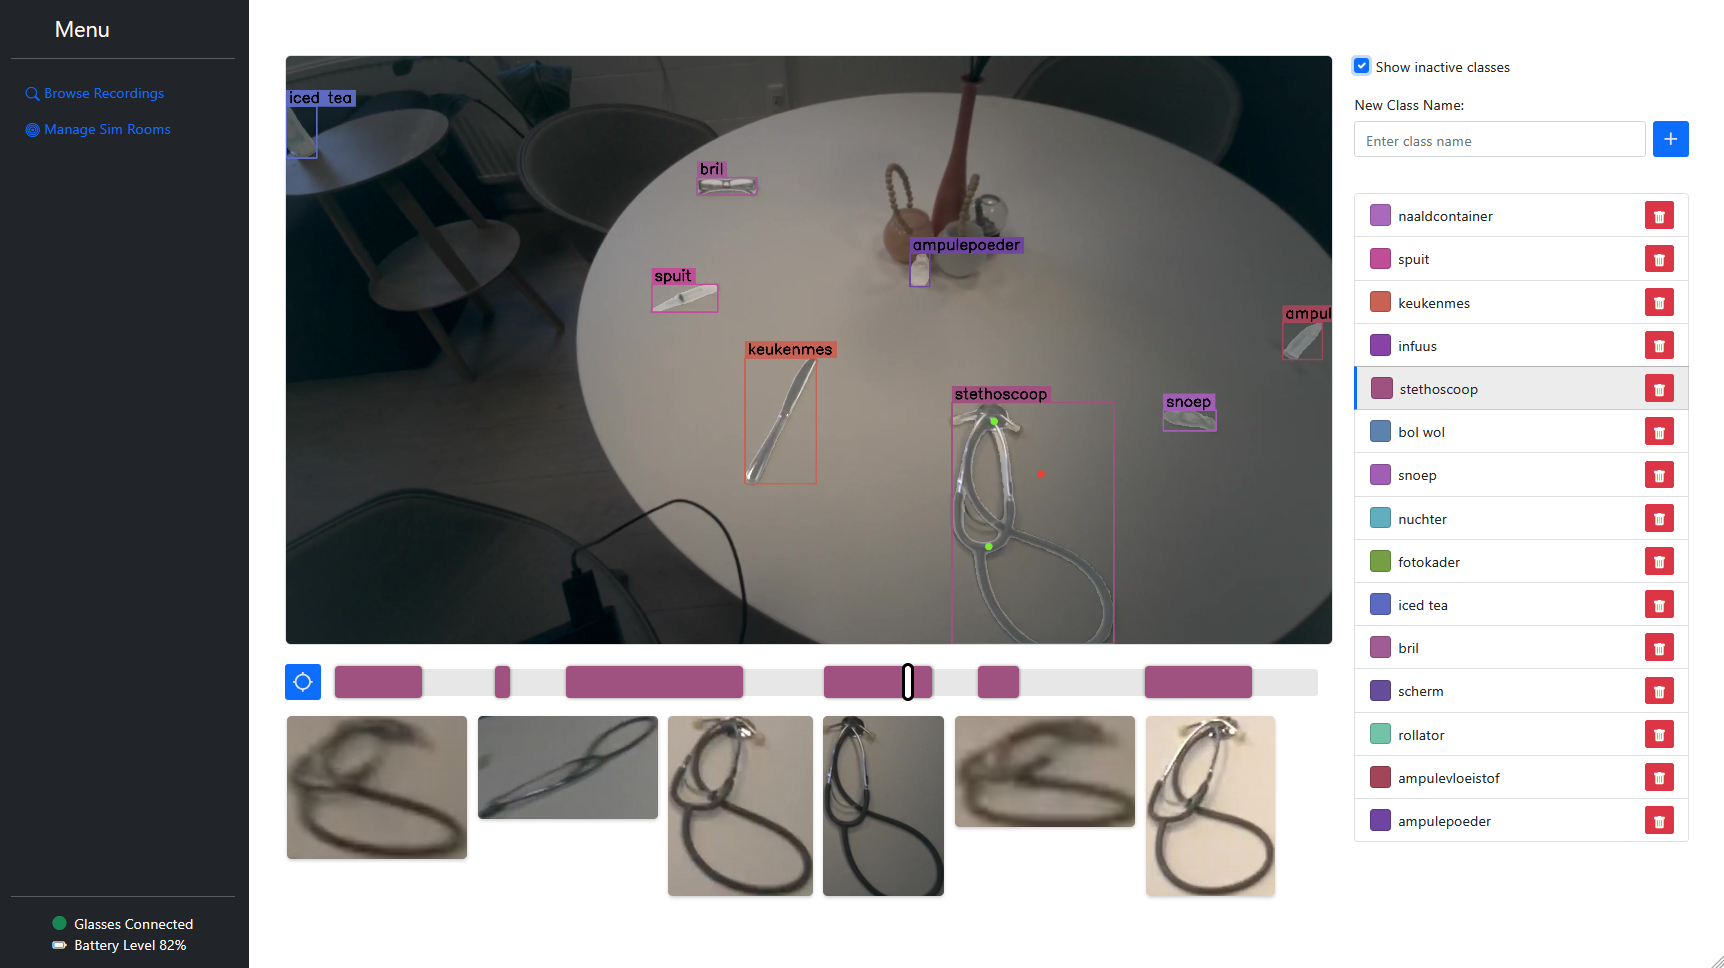
\includegraphics[width=1\textwidth]{labeler.png}
  \caption[]{\label{fig:labeler} Een screenshot van de labeling-tool met vier onderdelen: de labeling-canvas, de tijdlijn, de objectenlijst rechts, en een lijst van gemaakte annotaties onderaan. In dit voorbeeld is het object `stethoscoop' geselecteerd. }
\end{figure}

Eenmaal de labeling-tool geopend is, zien we een pagina met vier onderdelen (zie figuur \ref{fig:labeler}).
Linksboven zien we het `labeling-canvas', waar de huidige geselecteerde frame van de opname wordt getoond. Onder het canvas is er een tijdlijn die aangeeft waar we ons bevinden in de opname. De tijdlijn markeert ook welke frames het gevolgde object bevatten. 
Binnen deze canvas kunnen we objecten labelen door eerst een object in de lijst rechts te selecteren, en vervolgens te klikken op het canvas.
Hierbij kunnen we een linkermuisklik gebruiken om aan te geven welke delen van de afbeelding deel uitmaken van het object dat we willen labelen (zie de stethoscoop in figuur \ref{fig:labeler}). Met de rechtermuisklik geven we aan welke regio's buiten het object vallen.
Deze zijn respectievelijk gemarkeerd met een groene en een rode stip. Als we met de muis over een stip gaan, wordt deze gemarkeerd. Vervolgens kunnen we erop klikken om de stip te verwijderen.
Na elke muisklik worden het masker en de bijbehorende \textit{bounding box} automatisch geüpdatet om feedback te geven aan de gebruiker.

Onder de tijdlijn zien we een reeks annotaties die we hebben gemaakt, van links naar rechts gesorteerd op tijd. Men kan op deze annotaties klikken om naar de bijbehorende frame te gaan, en ze ook verwijderen door met de muis erover te gaan en op de rode knop te klikken.
Indien men alle stippen verwijdert, wordt de annotatie ook verwijderd.
Eens we tevreden zijn met de annotaties, kunnen we op de blauwe `tracking'-knop klikken aan de linkerkant van de tijdlijn.
Dit start de automatische tracking van het huidige geselecteerde object doorheen de opname, zoals getoond in figuur \ref{fig:labeler-tracking}. 

\begin{figure}[H]
  \centering
  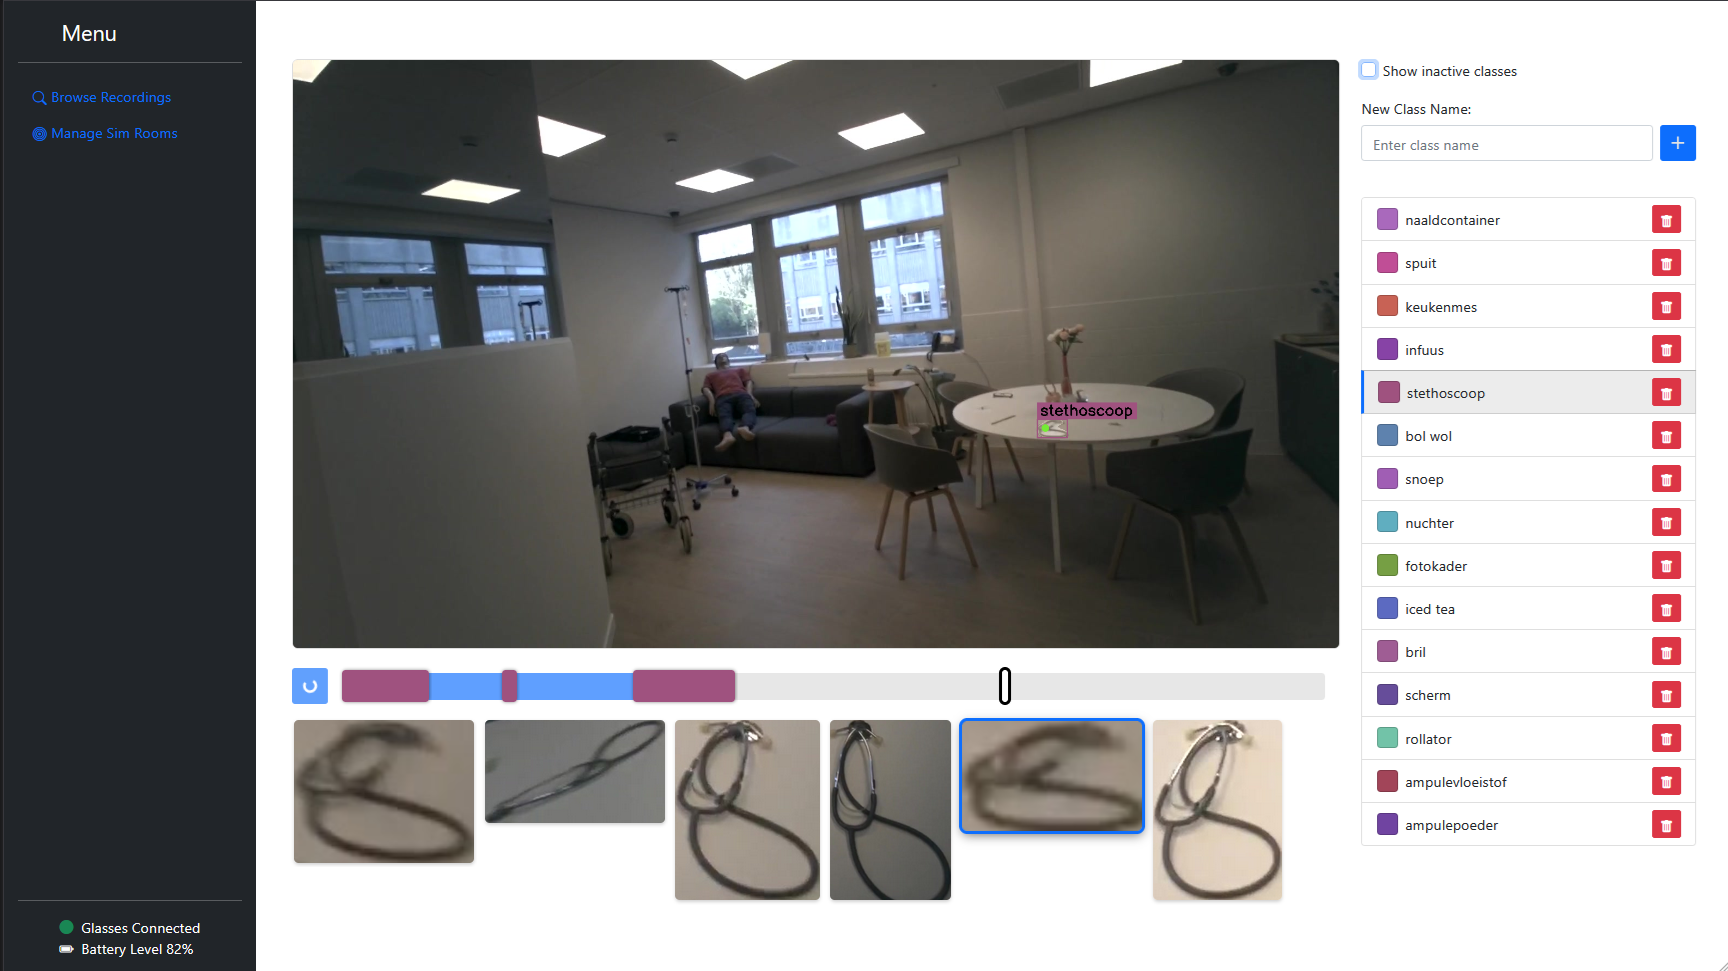
\includegraphics[width=1\textwidth]{labeler-tracking.png}
  \caption[]{\label{fig:labeler-tracking} In deze screenshot zien we dat er een tracking-opdracht gaande is. Hier is ook de optie `Show inactive classes' uitgevinkt, waardoor enkel het actieve object wordt getoond. }
\end{figure}

Uit praktische overweging worden niet alle frames bekeken binnen een tracking-opdracht. Een annotatie wordt als basis gebruikt voor tracking, en wanneer het object voor een bepaalde tijd uit het beeld verdwijnt, wordt de trackingopdracht stopgezet tenzij er nog annotaties overblijven.
Over het algemeen hebben we slechts één annotatie nodig voor elk gedeelte van de video waarin het object voortdurend in beeld is. Soms zijn echter meerdere annotaties per gedeelte nodig om het trackingresultaat te optimaliseren.
Het specifieke algoritme dat bedacht werd voor de tracking komt aan bod in de technische sectie van dit onderdeel.
Tenslotte bestaat de mogelijkheid dat er veel objecten in beeld zijn waardoor maskers, bounding boxes en labels elkaar overlappen. Om deze reden kunnen we rechtsboven een optie `Show inactive classes', uitvinken om enkel het actieve object te tonen in het canvas.

\subsection{Analyse van Eyetracking-Opnames}

Hoewel het aanvankelijk de bedoeling was, werd in de context van deze bachelorproef, geen werkende analyse-tool ontwikkeld maar enkel een proof-of-concept.
De labeling-tool was in dit opzicht de belangrijkste component, omdat deze de labels genereert die nodig zijn voor de analyse.
Aangezien de het hier enkel een proof-of-concept betrof, werd hier ook geen pagina voor ontwikkeld.
Indien men in de toekomst een betrouwbaar analysemodel kan ontwikkelen, bestaat de mogelijkheid om een nieuwe pagina te maken die de resultaten van de analyses toont.
Naast de pagina zelf dient dan ook een bijbehorende optie in de navigatiekolom aangemaakt te worden.
De analyses die uitgevoerd werden in deze bachelorproef komen aan bod in Hoofdstuk~\ref{ch:experiment}.

\section{Technische Specificaties}

We hebben het gehad over de features van de applicatie vanuit het perspectief van een gebruiker.
In deze sectie gaan we dieper in op de technische aspecten van de applicatie, 
met als doel de keuzes te verduidelijken en eventuele nieuwe developers wegwijs te maken in de codebase.

\subsection{Softwarearchitectuur}

Voor de ontwikkeling van de applicatie werd een lichtgewicht, modulaire softwarestack gekozen, afgestemd op de specifieke noden van het project.
Er is geopteerd voor een web-applicatie die via een browser toegankelijk is en lokaal kan draaien op een laptop (met een degelijke grafische kaart) of een desktop computer.

\begin{itemize}
    \item \textbf{Backend Framework:} Python met \texttt{FastAPI} werd gekozen omwille van zijn gebruiksvriendelijkheid, asynchrone mogelijkheden (belangrijk voor I/O-intensieve taken zoals data-import en analyse), automatische documentatie en type hinting-integratie.
    \item \textbf{Frontend Aanpak:} In plaats van een zwaar JavaScript-framework, werd geopteerd voor \texttt{HTMX}. Dit laat toe om dynamische interacties te bouwen door HTML direct uit te wisselen met de server, wat de complexiteit van de frontend aanzienlijk reduceert. \texttt{Jinja2} dient als templating engine om deze HTML server-side te genereren. Tenslotte werd \texttt{Bootstrap} gebruikt voor de opmaak van de applicatie.
    \item \textbf{Database:} Een \texttt{SQLite} database werd geselecteerd vanwege de eenvoud en het feit dat de applicatie bedoeld is voor lokaal gebruik, waardoor een complexe database server overbodig is. \texttt{SQLAlchemy} werd ingezet als ORM (Object-Relational Mapping) voor een gestructureerde interactie met de database vanuit Python.
    \item \textbf{Hardware Communicatie:} Voor de interactie met de Tobii Pro Glasses 3 werd de officiële \texttt{g3pylib} SDK gebruikt, die toegang biedt tot opnames en statusinformatie via de WiFi-verbinding.
    \item \textbf{Development \& Kwaliteitsborging:} \texttt{Poetry} werd gebruikt voor dependency management. Strikte type hinting met \texttt{Mypy} en code linting/formatting met \texttt{Ruff} dragen bij aan de robuustheid en onderhoudbaarheid van de code. \texttt{Docker} werd ingezet om de applicatie te containeriseren, wat zorgt voor een consistente uitvoeringsomgeving en eenvoudige deployment.
\end{itemize}

% TODO: voetnoten toevoegen naar SDK en stuff

Deze keuzes resulteerden in een applicatie die relatief eenvoudig te onderhouden en verder te ontwikkelen is, conform de doelstelling om iteratieve verbeteringen in volgende bachelorproeven mogelijk te maken.
Er werd gewerkt met een gelaagde architectuur om een duidelijke scheiding van verantwoordelijkheden (Separation of Concerns) te waarborgen en onderhoud en testing te vereenvoudigen. 
De data en requests vloeien doorgaans van de \texttt{frontend} via de \texttt{routes} naar de \texttt{services}, die vervolgens de \texttt{repositories} aanroepen voor databasetoegang (zie figuur \ref{fig:software-architectuur}).

\begin{figure}[H]
  \centering
  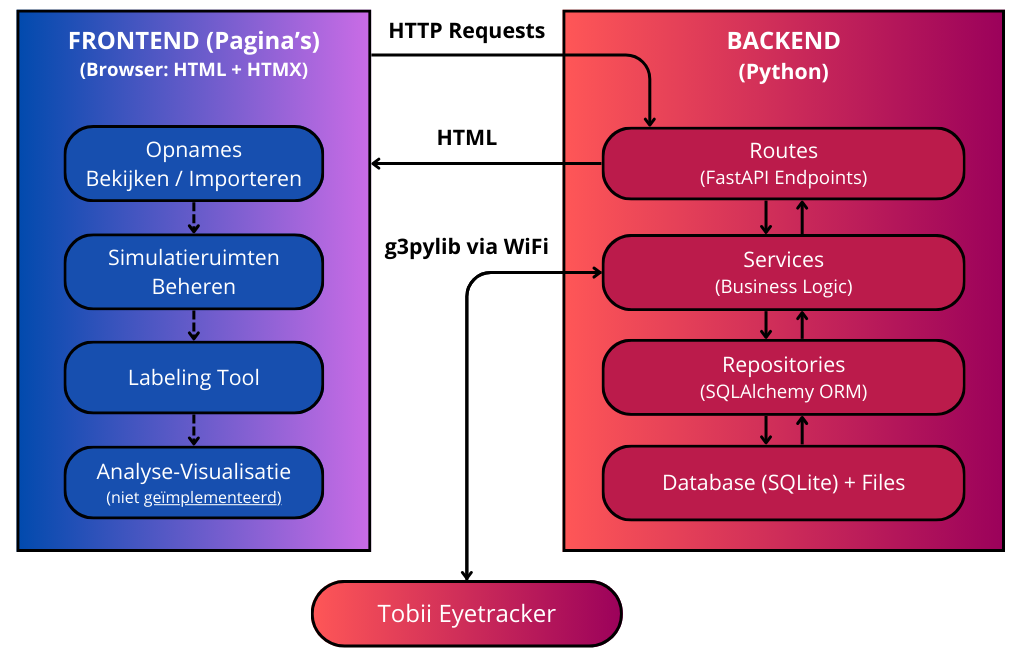
\includegraphics[width=0.8\textwidth]{software-architectuur.png}
  \caption[]{\label{fig:software-architectuur} Software-architectuur van de applicatie. De applicatie is opgebouwd uit verschillende lagen die elk hun eigen verantwoordelijkheden hebben. }
\end{figure}
% Link naar canva: https://www.canva.com/design/DAGmr8n_Umg/6k1gqiCpq2hON75Jq9H17Q/edit?utm_content=DAGmr8n_Umg&utm_campaign=designshare&utm_medium=link2&utm_source=sharebutton

\subsubsection{Frontend (HTML, HTMX, en Jinja2)}

De gebruikersinterface (UI) wordt weergegeven in de browser en is opgebouwd uit HTML-pagina's die server-side worden gegenereerd met behulp van de \texttt{Jinja2} templating engine.
Deze engine maakt het mogelijk om inhoud (data vanuit de Backend) te integreren in de HTML-pagina's door gebruik te maken van variabelen en controle-structuren.
Voor de dynamische aspecten van de applicatie, waaronder het bijwerken van de UI zonder de volledige pagina te herladen, wordt \texttt{HTMX} ingezet.

\texttt{HTMX} maakt het mogelijk om via HTML-attributen oproepen te doen naar de backend (vb: als een knop wordt ingedrukt).
De backend genereert vervolgens het gevraagde HTML-fragment---zoals een tabel met opnames of een lijst van objecten---die HTMX vervolgens injecteert in de huidige pagina.
Op deze manier kunnen eenvoudige interacties worden gerealiseerd zonder de noodzaak van een volledig JavaScript-framework zoals React of Vue.js.

Binnen de `Browse Recordings'-en `Manage Sim Rooms'-pagina's is HTMX grotendeels voldoende, maar toch valt JavaScript niet volledig te vermijden.
De labeling-tool vergt immers complexe interacties die niet eenvoudig gerealiseerd kunnen worden met enkel HTML en HTMX.
Zo werd de labeling-tool opgesplitst in vijf componenten die elk hun eigen verantwoordelijkheden hebben:
\begin{itemize}
    \item De \textbf{labeling-canvas} die de huidige frame toont en het mogelijk maakt om objecten te labelen.
    \item De \textbf{tijdlijn} die de voortgang van de opname toont en het mogelijk maakt om naar een specifieke frame te navigeren.
    \item De \textbf{objectenlijst} die de beschikbare objecten toont en het mogelijk maakt om objecten te beheren en te selecteren.
    \item De \textbf{annotatielijst} die de gemaakte annotaties van het momenteel geselecteerde object toont.
    \item De \textbf{labeling settings} die instellingen van de labeling-tool toont (`Show inactive classes').
\end{itemize}
Elk van deze componenten communiceert apart via HTMX-attributen met de backend, en kunnen onafhankelijk van elkaar worden geladen.
Wanneer toch communicatie nodig is tussen de componenten, gebeurt dit via \texttt{Events} die door de componenten worden uitgezonden en opgevangen.
Een voorbeeld hiervan is wanneer de gebruiker klikt op de tijdlijn om naar een specifieke frame te navigeren.
De tijdlijn stuurt een event naar de labeling-canvas, die vervolgens een oproep doet naar de backend om de juiste frame op te halen.

Aangezien het gaat om een single-user applicatie, is het toch mogelijk om een groot deel van de logica over te dragen aan de backend.
De frontend is dus voornamelijk verantwoordelijk voor de presentatie van de data en de interactie met de gebruiker.
De backend is verantwoordelijk voor de verwerking van de data, en het bijhouden van de status van de applicatie (de huidige frame, de geselecteerde objecten, de machine-learning modellen, etc.).

\subsubsection{Backend (Python met FastAPI)}

De backend, geschreven in Python met het \texttt{FastAPI} framework, is verantwoordelijk voor het verwerken van requests, 
het uitvoeren van de businesslogica, en de interactie met de datalaag en externe hardware.

\paragraph{Routes (FastAPI Endpoints)}
De \texttt{routes} definiëren de API-endpoints waarnaar de frontend requests stuurt.
Deze laag ontvangt HTTP-requests, valideert inkomende data 
(via Pydantic modellen die FastAPI automatisch uit request bodies of query parameters haalt), 
roept de juiste methoden aan in de \texttt{services}-laag, en formatteert de respons. 
Voor HTMX-requests is dit typisch een HTML-fragment gerenderd met Jinja2; voor andere endpoints kan dit JSON zijn 
(bv. het ophalen van annotatiepunten voor de labeler).

\paragraph{Services (Business Logic)}
De \texttt{services}-laag bevat de kernlogica van de applicatie.
Services coördineren operaties en implementeren de business rules. 
Ze zijn ontkoppeld van de HTTP-laag en de directe database-implementatie. 
In plaats daarvan gebruiken ze methoden uit de \texttt{repositories}-laag voor datatoegang- en persistentie, 
en kunnen ze andere utilities of externe bibliotheken aanroepen (bv. \texttt{g3pylib} voor communicatie met de Tobii-bril, of \texttt{SAM2ImagePredictor} voor segmentatie).

\paragraph{Repositories (Data Access)}
De \texttt{repositories}-laag vormt de abstractielaag boven de database en het filesysteem.
Het bevat alle logica voor het ophalen, opslaan, en beheren van data in de \texttt{SQLite} database via \texttt{SQLAlchemy} ORM.
Ook bevat het logica voor het beheren van bestanden op de schijf, zoals resultaten van de labeling-tool of de video-opnames.
Dit zorgt ervoor dat de \texttt{services}-laag onafhankelijk is van de specifieke database-implementatie.

\subsection{Backend van de Labeling Tool en Tracking-logica}
\label{sec:labeling-tool-logic}

In deze sectie gaan we dieper in op wat er in de achtergrond gebeurt wanneer de gebruiker objecten labelt in de labeling-tool.

\subsubsection{Decoderen van Video-opnames}

Alvorens de gebruiker kan beginnen met labelen, moeten eerst de frames van de opname worden geëxtraheerd.
Op deze manier moeten niet alle frames in het geheugen geladen worden, wat onmogelijk zou zijn voor lange opnames.
Ook neemt het enige tijd om een enkele frame te extraheren uit een video-opname, wat de gebruikerservaring zou beïnvloeden.
Voor het decoderen van een opname wordt gebruik gemaakt van \texttt{ffmpeg}, een populaire open-source tool die verschillende 
functies biedt voor het verwerken van video- en audiobestanden.
Zo worden alle afzonderlijke frames opgeslagen in een map, met als naam het indexnummer van het frame.

Doorheen zowel de applicatie als de analyses is het heel belangrijk om dezelfde video-decoder te gebruiken.
Verschillende decoders (zoals \texttt{ffmpeg} of \texttt{OpenCV}) kunnen andere frame- en tijdsindexering gebruiken.
Als men bijvoorbeeld een frame-index van 100 opgeeft, kan dit in de ene decoder overeenkomen met de 100ste frame, terwijl het in een andere decoder de 101ste frame is.
Dit kan leiden tot inconsistenties in de resultaten van de analyses, en dus werd er gekozen om steeds \texttt{ffmpeg} te gebruiken.

\subsubsection{Annotaties en Tracking}

Voor een beter begrip van het waarom van manuele annotaties, en hoe de geautomatiseerde tracking werkt, moeten we eerst begrijpen hoe het achterliggende machine-learning model werkt.
Er werd gekozen om het Segment Anything Model 2 (SAM2) van Meta te gebruiken, dat in staat is om objecten te segmenteren (een masker genereren) in zowel een afbeelding als een video.

Via het `promptable-segmentation'-mechanisme van SAM2 kunnen we een object segmenteren door een aantal punten te geven die het object beschrijven.
Men kan een positief punt geven dat `binnen' het object ligt (voorgesteld door een 1), en een negatief punt dat `buiten' het object ligt (voorgesteld door een 0).
Zo krijgen we een annotatie die uit meerdere punten bestaat (zie figuur \ref{fig:annotation}).

\begin{figure}[H]
  \centering
  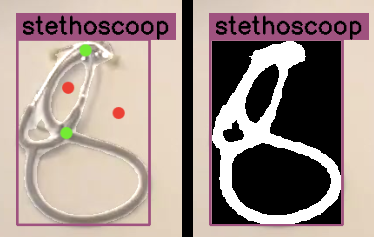
\includegraphics[width=0.8\textwidth]{annotation.png}
  \caption[]{\label{fig:annotation} Links een annotatie met een aantal positieve (groene) en negatieve (rode) punten zoals zichtbaar in de labeling-tool. Rechts het overeenkomstig masker dat werd gegenereerd door SAM2. }
\end{figure}

De manuele annotaties vormen de basis voor de automatische tracking van het object doorheen de opname.
Zoals eerder vermeld, worden niet alle frames bekeken binnen deze tracking-opdracht.
Het frame-per-frame verwerken van een volledige video-opname is immers onnodig (wanneer een object voor een lange tijd niet in beeld is) en tijdrovend.

Om de tracking efficiënt uit te voeren, fungeert elke manuele annotatie als een startpunt. 
De \texttt{TrackingJob} klasse initieert vanuit deze `ankerpunten' het trackingproces, zoals geïmplementeerd in de run methode:

\begin{listing}[H]
  \begin{minted}{python}
    def run(self) -> None:
      self.initialize()

      annotations_frame_idx = [annotation.frame_idx for annotation in self.annotations]
      last_tracked_annotation = -1

      while last_tracked_annotation != len(self.annotations) - 1:
          start_frame_idx = annotations_frame_idx[last_tracked_annotation + 1]
          self.progress = start_frame_idx / self.frame_count

          # Voorwaarts tracken tot tracking verlies:
          list(self.track_until_loss(start_frame_idx, reverse=True))

          # Achterwaarts tracken tot tracking verlies:
          for frame_idx in self.track_until_loss(start_frame_idx):
              self.progress = frame_idx / self.frame_count
              if frame_idx in annotations_frame_idx:
                  last_tracked_annotation = annotations_frame_idx.index(frame_idx)
  \end{minted}
  \caption[Kernlogica van de \texttt{TrackingJob} voor efficiënte verwerking]{
    De \texttt{run} methode van \texttt{TrackingJob} itereert over de gesorteerde manuele annotaties en start vanuit elk ankerpunt een 
    gelokaliseerd tracking-proces om de rekentijd te beperken.
  }
\end{listing}

De strategie is als volgt:
\begin{enumerate}
\item De \texttt{TrackingJob} ontvangt een lijst van manuele annotaties, die eerst gesorteerd worden op frame-index.
\item Vervolgens wordt er over deze annotaties geïtereerd. Voor elke nog niet verwerkte annotatie (\texttt{start\_frame\_idx}) 
wordt de functie \texttt{track\_until\_loss} aangeroepen, eerst in achterwaartse richting (\texttt{reverse=True}) en daarna in voorwaartse richting.
\item Dit zorgt ervoor dat de tracking zich vanuit elk betrouwbaar, manueel gelabeld punt propageert over videosegmenten waar het object vermoedelijk aanwezig is. 
Dit reduceert het totaal aantal te verwerken frames aanzienlijk.
\end{enumerate}

De kern van het daadwerkelijke volgen binnen deze segmenten zit in de \texttt{track\_until\_loss} methode. 
Deze methode maakt gebruik van de \texttt{propagate\_in\_video} functionaliteit van de \texttt{SAM2VideoPredictor}.

\begin{listing}[H]
  \begin{minted}{python}
    def track_until_loss(
        self, start_frame_idx: int, reverse: bool = False
    ) -> Generator[int, None, None]:
        tracking_loss = 0 # Teller voor het aantal frames zonder tracking

        with torch.amp.autocast("cuda"):
            for (
              out_frame_idx, _, out_mask_logits
            ) in self.video_predictor.propagate_in_video(
                inference_state=self.inference_state,
                start_frame_idx=start_frame_idx,
                reverse=reverse,
            ):
                yield out_frame_idx # Rapporteer de verwerkte frame index voor de progress bar

                mask_torch = out_mask_logits[0] > 0.5
                if mask_torch.any(): # Is er een masker getedecteerd?
                    tracking_loss = 0 # Reset teller bij succesvolle tracking

                    # ... (opslaan van resultaten: masker, box, roi) ...

                    file_path = self.results_path / f"{out_frame_idx}.npz"
                    np.savez_compressed(
                        file_path,
                        # ... (data)
                    )
                else:
                    tracking_loss += 1 # Verhoog teller bij mislukte tracking

                if tracking_loss >= self.GRACE_PERIOD: # Tolerantie overschreden?
                    break # Stop tracking in deze richting

  \end{minted}
  \caption[Gelokaliseerde tracking met tolerantieperiode]{
    De \texttt{track\_until\_loss} methode propageert het masker frame-per-frame binnen een beperkt segment. 
    De \texttt{GRACE\_PERIOD} helpt om de tracking robuust te houden tegen kortstondige detectieproblemen binnen dit segment.
  }
\end{listing}

\paragraph{Waarom geen FastSAM?}

Men zou zich kunnen afvragen waarom het FastSAM-model niet werd gebruik, aangezien het ook in staat is om objecten te segmenteren in video-opnames en bovendien veel sneller is.
Het probleem is dat de gegenereerde maskers van FastSAM minder nauwkeurig zijn dan die van SAM2 \autocite{Zhao2023}. 
Aangezien het om labeling gaat, is het belangrijk dat de maskers zo nauwkeurig mogelijk zijn.
Het is mogelijk dat dit verschil in de context van deze bachelorproef niet zo belangrijk is, maar het zou onnauwkeurig zijn om dit te stellen zonder de verschillen in detail te analyseren.
Hoewel het testen van FastSAM binnen de labeling-tool niet verder werd uitgewerkt, werd dit model wel gebruikt voor de analyses in Hoofdstuk~\ref{ch:experiment}.
Zo zijn er voorbeelden van het gebruik van beide modellen binnen de codebase terug te vinden, en kan de labeling-tool overschakelen naar FastSAM indien gewenst.

\subsubsection{Prestaties en Geheugenverbruik}

Belangrijke overwegingen bij het implementeren van de applicatie in het Zorglab zijn de hardwarevereisten.
Het Zorglab is uitgerust met een computer met een krachtige CPU (Central Processing Unit) en 32GB RAM, maar heeft momenteel geen GPU (Graphics Processing Unit).
Daarom is het interessant om te kijken wat de vereisten zijn voor een vlotte werking van de applicatie.
Hier zullen we het specifiek hebben over SAM2, maar in hoofdstuk \ref{ch:experiment} komen ook de modellen van de analyses aan bod.

De ontwikkeling van de applicatie, inclusief alle analyses, werd uitgevoerd op een computer met de volgende specificaties:
\begin{itemize}
    \item \textbf{Processor:} Ryzen 7 7700X @ 4.50 GHz (8 cores)
    \item \textbf{Geheugen:} 32GB DDR5
    \item \textbf{Grafische Kaart:} NVIDIA GeForce RTX 4090 (24GB VRAM)
    \item \textbf{Opslag:} 1TB M.2 SSD
\end{itemize}

De machine in het Zorglab is een Dell Precision 7550 met de volgende specificaties:
\begin{itemize}
    \item \textbf{Processor:} Intel Core i9-10885H CPU @ 2.40 GHz (16 cores)
    \item \textbf{Geheugen:} 32GB
    \item \textbf{Grafische Kaart:} Geen
\end{itemize}

\paragraph{Verschil tussen CPU en GPU}
Voor taken binnen machine-learning, zoals de hier toegepaste beeldsegmentatie, is een GPU significant sneller dan een CPU. 
Een CPU specialiseert zich in het sequentieel uitvoeren van een beperkt aantal complexe taken. 
Een GPU daarentegen is ontworpen met duizenden kleinere cores (de RTX 4090 heeft er bijvoorbeeld 16,384) 
om een grote hoeveelheid relatief eenvoudigere taken parallel uit te voeren. 
Dit parallellisme is ideaal voor de matrixoperaties die de ruggengraat vormen van neurale netwerken zoals SAM2.

Niet enkel het aantal cores is bepalend, maar ook de hoeveelheid en snelheid van het geheugen op de GPU (VRAM).
Zowel het model zelf (de parameters of 'gewichten') als de te verwerken data (in dit geval de videoframes) moeten tegelijkertijd 
in het VRAM geladen kunnen worden voor efficiënte verwerking.
Pogingen om dergelijke modellen uitsluitend op een CPU uit te voeren, resulteren in onpraktisch lange verwerkingstijden, 
waardoor de interactiviteit van de labeling tool verloren zou gaan.

\paragraph{Analyse van de prestaties}

Het SAM2-model komt in vier verschillende varianten, elk met een andere hoeveelheid parameters en dus ook andere geheugenvereisten.
Via de \texttt{torch.profiler} module werd het geheugengebruik van elk model gemeten tijdens het laden van de parameters.
De resultaten hiervan zijn als volgt:

\begin{itemize}
    \item \texttt{sam2.1\_hiera\_large.pt}: 1000 MB
    \item \texttt{sam2.1\_hiera\_base\_plus.pt}: 450 MB
    \item \texttt{sam2.1\_hiera\_small.pt}: 315 MB
    \item \texttt{sam2.1\_hiera\_tiny.pt}: 288 MB
\end{itemize}

Aangezien geheugenvereisten relatief laag zijn, werd besloten om het grootste model te gebruiken, dat ook de beste resultaten oplevert.

Naast de modelparameters is het ook belangrijk het geheugengebruik te meten bij de tracking-opdracht.
Zo werd doorheen een tracking-opdracht gemeten hoeveel videogeheugen er werd gebruikt door het SAM2 model.
Het ging om een totaal van 360 getrackede frames aan een snelheid van 10.5fps, met een piek geheugenverbruik van 1599 MB (zie figuur \ref{fig:sam-mem-usage}).

\begin{figure}[H]
  \centering
  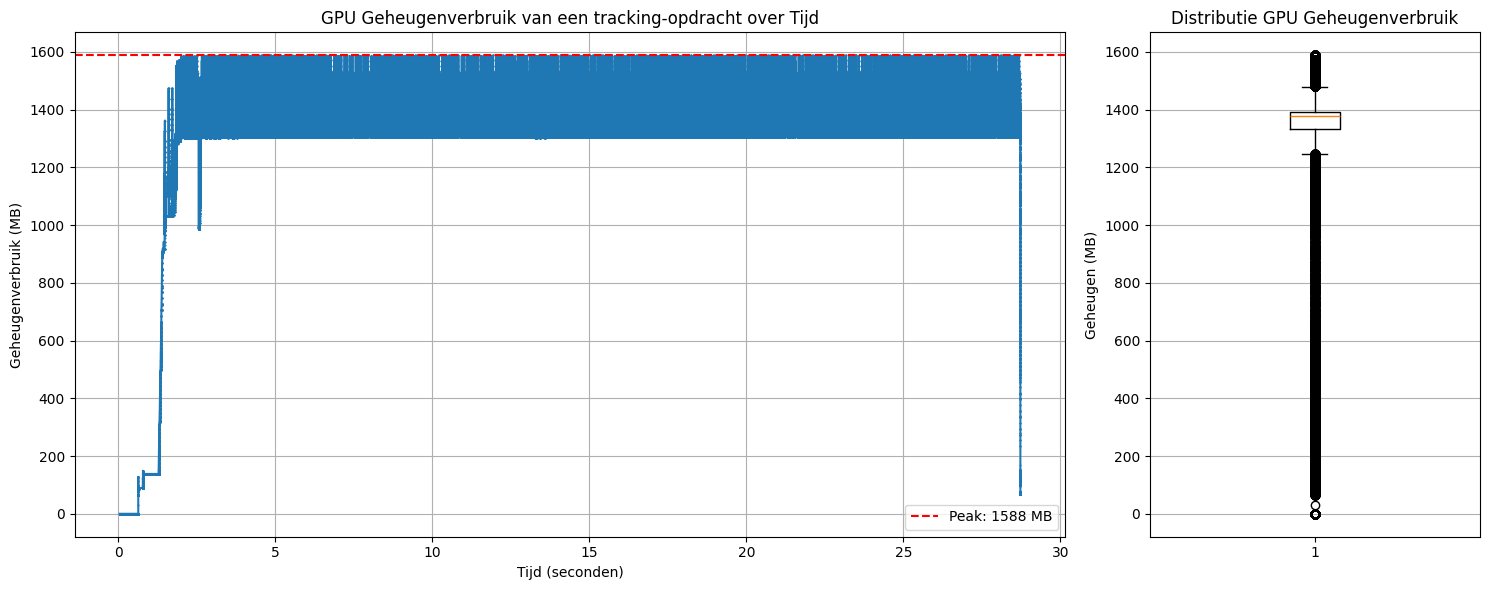
\includegraphics[width=1\textwidth]{sam_mem_usage.png}
  \caption[]{\label{fig:sam-mem-usage} 
  Het geheugengebruik van SAM2 tijdens een tracking-opdracht. Links het cumulatieve geheugengebruik doorheen de tijd met een piek van 1599MB, rechts een boxplot van het geheugengebruik met een gemiddelde van 1374 MB. }
\end{figure}

Deze analyses zijn terug te vinden in de file \texttt{experiment/12\_performance.ipynb} in de Git repository.

\subsubsection{Optimalisatie van Geheugenbeheer in de SAM2-bibliotheek}

Tijdens de ontwikkeling van de tracking-functionaliteit werd een probleem met 
toenemend GPU-geheugenverbruik in de originele SAM2-bibliotheek van Meta geïdentificeerd \autocite{Hu2024facebookresearch}. 
Bij langdurige tracking-opdrachten, bleek dat de bibliotheek intermediaire 
resultaten of toestanden van reeds verwerkte frames in het GPU-geheugen vasthield. 
Dit leidde tot een lineaire toename van het VRAM-gebruik naarmate de tracking vorderde. 
Uiteindelijk kon dit de beschikbare GPU-geheugenlimiet overschrijden, en zo doende resulteren in een crash van de applicatie. 

Om dit probleem aan te pakken en het GPU-geheugenverbruik te stabiliseren, werd er een fork gemaakt van de originele 
SAM2-bibliotheek waarin een aanpassing is doorgevoerd \autocite{Hu2025ilianbronchart}.
De oplossing is geïnspireerd door een Github-issues comment \autocite{heyoeyo2024comment}. 

De volgende code-snippet bevat de logica die werd toegevoegd binnen de propagatielus van de video-predictor:
\begin{listing}[H]
  \begin{minted}{python}
  # Fragment uit de aangepaste SAM2VideoPredictor binnen de video propagatie lus
  # Bepaal de dictionary waar frame outputs worden opgeslagen
  obj_output_dict = inference_state["obj_wise_inference_states"][obj_id]
  storage_key = "non_cond_frame_outputs"
  obj_specific_storage_key = "output_dict_per_obj"

  # Identificeer oude frames die verwijderd moeten worden
  if reverse: # Bij achterwaarts tracken
      # Verwijder frames die te ver vooruit liggen
      newest_allowed_idx = frame_idx + 16 # Behoud een buffer van 16 frames
      all_frame_idxs = obj_output_dict[storage_key].keys()
      old_frame_idxs = [idx for idx in all_frame_idxs if idx > newest_allowed_idx]
  else: # Bij voorwaarts tracken
      # Verwijder frames die te ver achterliggen
      oldest_allowed_idx = frame_idx - 16 # Behoud een buffer van 16 frames
      all_frame_idxs = obj_output_dict[storage_key].keys()
      old_frame_idxs = [idx for idx in all_frame_idxs if idx < oldest_allowed_idx]

  # Verwijder de geïdentificeerde oude frames uit de cache
  for old_idx in old_frame_idxs:
      obj_output_dict[storage_key].pop(old_idx, None) # Verwijder uit algemene cache
      # Verwijder ook uit object-specifieke caches indien aanwezig
      for objid_iter in inference_state[obj_specific_storage_key].keys():
          if old_idx in inference_state[obj_specific_storage_key][objid_iter][storage_key]:
              inference_state[obj_specific_storage_key][objid_iter][storage_key].pop(old_idx, None)
  \end{minted}
  \caption[Geheugenoptimalisatie in SAM2 door caching van frame outputs]{Toegevoegde logica om gecachte frame-specifieke outputs selectief te verwijderen, waardoor het GPU-geheugengebruik tijdens lange tracking-sessies constant blijft.}
  \label{lst:sam2-memory-fix}
\end{listing}

De oplossing werkt als volgt:
\begin{enumerate}
  \item De code richt zich op specifieke dictionaries binnen de \texttt{inference\_state} waar frame-gerelateerde data worden opgeslagen.
  \item Er wordt een buffer rond de huidige \texttt{frame\_idx} gedefinieerd. Data van frames die buiten dit venster vallen, worden beschouwd als `oud' en komen in aanmerking voor verwijdering.
  \item De geïdentificeerde \texttt{old\_frame\_idxs} worden vervolgens uit de relevante cache-dictionaries verwijderd. Dit gebeurt zowel voor de algemene frame outputs als voor de object-specifieke outputs.
\end{enumerate}
Merk op dat de buffer van 16 frames hier hardgecodeerd is. 
In de toekomst kan het nuttig zijn om deze waarde aanpasbaar te maken door middel van een configuratieparameter binnen de \texttt{SAM2VideoPredictor} klasse.

\subsection{Omgaan met Blikdata}
\label{sec:omgaan-met-blikdata}

Om de analyses in Hoofdstuk~\ref{ch:analyse} te vergemakkelijken, en voor het bouwen van de grondwaarheid in Hoofdstuk~\ref{ch:grondwaarheid}, biedt de applicatie 
in de service-laag (geïmplementeerd in \texttt{src.api.services.gaze\_service}) ook functionaliteit om de blikdata van de eyetracker te verwerken.
Deze functionaliteit omvat het laden, verwerken en synchroniseren van de blikdata met de videoframes.
Hier worden de kernstappen van deze functionaliteit besproken.

\subsubsection{Parseren van Blikdatabestanden}

De blikdata van de eyetracker worden opgeslagen in een \texttt{.tsv}-bestand.
Hoewel men er kan van uitgaan dat het hier om tab-separated values gaat (tsv), blijkt dit niet het geval te zijn.
In de werkelijkheid bestaan deze bestanden uit een reeks van \texttt{json}-objecten, waarbij elke regel metadata bevat over een bepaald blikpunt.
De \texttt{parse\_gazedata\_file} functie is verantwoordelijk voor het inlezen van de bestanden, 
en levert een lijst aan \texttt{GazeData} objecten op.

Het volgende is een voorbeeld van een regel uit een blikdatabestand:
\begin{listing}[H]
  \begin{minted}{python}
    {
        "type": "gaze",
        "timestamp": 0.014574,
        "data": {
            "gaze2d": [
                0.42802076888650348,
                0.59985904570034698
            ],
            "gaze3d": [
                5524.405064657687,
                -4220.9188210373977,
                38060.311822743075
            ],
            "eyeleft": {
                "gazeorigin": [
                    32.591088912983722,
                    -9.3800673986482224,
                    -28.144596430671765
                ],
                "gazedirection": [
                    0.14673772446588171,
                    -0.10725782137152362,
                    0.98334317507836977
                ],
                "pupildiameter": 3.078226794385742
            },
            "eyeright": {
                "gazeorigin": [
                    -28.884017016163959,
                    -9.1355755568510908,
                    -27.103885607429742
                ],
                "gazedirection": [
                    0.13854486333094154,
                    -0.11030711082172073,
                    0.98419391491045893
                ],
                "pupildiameter": 3.1712040692965147
            }
        }
    }
  \end{minted}
  \caption[Voorbeeld van een regel in een blikdatabestand]{
    Een voorbeeld van een regel in een blikdatabestand. 
    Het bevat metadata over de blikdata, zoals de tijdstempel, de 2D- en 3D-coördinaten van de blik, en de pupilgrootte.
  }
\end{listing}

Zoals men kan zien bevat elke regel van het bestand de volgende metadata, waarvan de uitleg afkomstig is uit de Tobii Glasses 3 Developer Guide \autocite{Tobii2023}:
\begin{itemize}
    \item \texttt{type}: het type van de data (in dit geval `gaze').
    \item \texttt{timestamp}: de tijdstempel van de data in seconden.
    \item \texttt{data}: een dictionary met de blikdata. Het is mogelijk dat deze leeg is wanneer er geen blikdata beschikbaar is. Het bevat de volgende velden:
    \begin{itemize}
      \item \texttt{gaze2d}: De 2D-coördinaten van de blik. Merk op dat dit genormaliseerde coördinaten zijn ten opzichte van de resolutie van de video-opname,
      waarbij (0, 0) de linkerbovenhoek van de video-opname is en (1, 1) de rechteronderhoek.
      \item \texttt{gaze3d}: Dit is een 3D-coördinaat in millimeters, dat de positie van de blik in de ruimte weergeeft tegenover de positie van de camera.
      \item \texttt{eyeleft} en \texttt{eyeright}: metadata over het linker en rechter oog, waaronder de oorsprong van de blik, de richting van de blik, en de pupilgrootte.
      Het is mogelijk dat één van deze velden leeg is wanneer er geen data beschikbaar is voor dat oog. Indien beide velden leeg zijn, betekent dit dat er geen blikdata beschikbaar zijn (het `data' veld is dan ook volledig leeg).
    \end{itemize}
\end{itemize}

\subsubsection{Converteren naar Bruikbare Blikpunten}

Nadat de ruwe blikdata zijn geparsed, worden deze verder verwerkt door de \texttt{get\_gaze\_points} functie.
Het resultaat van deze functie is een lijst van \texttt{GazePoint}-objecten, die elk een x- en y-coördinaat, 
de geschatte diepte, en de oorspronkelijke tijdstempel bevatten.
Hoewel de diepte binnen de analyses in Hoofdstuk~\ref{ch:analyse} niet verder wordt gebruikt, kan deze in de 
toekomst nuttig zijn voor andere analyses.

\begin{listing}[H]
  \begin{minted}{python}
    def get_gaze_points(
        gaze_data: list[GazeData], resolution: tuple[int, int]
    ) -> list[GazePoint]:
        gaze_points = [] 
        
        for data in gaze_data:
            if data.gaze2d is None:
                # Geen 2D-coördinaten beschikbaar, dus deze data is niet bruikbaar
                continue

            gaze_depth = None
            if data.gaze3d and data.eye_data_left and data.eye_data_right:
                eyeleft = data.eye_data_left
                eyeright = data.eye_data_right

                # Bereken de oorsprong van de blik als het 
                # gemiddelde van de oorsprong van beide ogen
                gaze_origin = (
                    np.add(eyeleft.origin, eyeright.origin) / 2
                    if (eyeleft and eyeright)
                    else eyeleft.origin
                    if eyeleft
                    else eyeright.origin
                )

                # Bereken de diepte van de blik als de 
                # euclidische afstand tussen de oorsprong en het 3D-punt
                gaze_depth = np.sqrt(np.sum((data.gaze3d - gaze_origin) ** 2, axis=0))

            # Denormaliseer de 2D-coördinaten naar pixelcoördinaten
            x = int(clamp(data.gaze2d[0], 0, 1) * resolution[1])
            y = int(clamp(data.gaze2d[1], 0, 1) * resolution[0])

            gaze_points.append(GazePoint(x, y, gaze_depth, data.timestamp))

        return gaze_points
  \end{minted}
  \caption[\texttt{get\_gaze\_points} functie]{
    De \texttt{get\_gaze\_points} functie verwerkt de ruwe blikdata en zet deze om naar bruikbare blikpunten.
    Het resultaat is een lijst van \texttt{GazePoint} objecten met de x- en y-coördinaten, de geschatte diepte, en de oorspronkelijke tijdstempel.
  }
\end{listing}

De functie heeft twee hoofddoelen:
\begin{enumerate}
  \item \textbf{Filteren van Ongeldige Data:} Blikregistraties waarbij geen \texttt{gaze2d}-coördinaten beschikbaar zijn, 
  worden genegeerd, omdat deze niet bruikbaar zijn voor 2D-analyse in het videobeeld.
  \item \textbf{Denormalisatie en Diepteberekening:}
    \begin{itemize}
      \item Een schatting van de diepte van het blikpunt (\texttt{gaze\_depth}) wordt berekend. 
        Indien data voor beide ogen beschikbaar zijn, wordt de 3D-oorsprong van de blik benaderd als 
        het gemiddelde van de \texttt{gazeorigin} van het linker- en rechteroog. 
        De diepte is dan de Euclidische afstand tussen dit gemiddelde oorsprongspunt en het geregistreerde \texttt{gaze3d}-punt.
      \item De genormaliseerde \texttt{gaze2d}-coördinaten (x, y) worden omgezet naar absolute pixelcoördinaten 
        ten opzichte van de resolutie van de video-opname. 
        Hierbij wordt gebruik gemaakt van de \texttt{clamp}-functie om te verzekeren dat de coördinaten 
        binnen de grenzen van de videoframe blijven alvorens te vermenigvuldigen met de respectievelijke breedte en hoogte.
    \end{itemize}
\end{enumerate}

\subsubsection{Synchronisatie van Blikpunten met Videoframes}

Een belangrijke stap voor analyse is het correct toewijzen van de continue stroom van blikpunten aan de verschillende videoframes.
De Tobii Pro Glasses 3 registreert blikdata met hogere frequentie (50Hz) dan de videoframerate (25fps).
Dit betekent dat er meerdere blikpunten kunnen corresponderen met een enkele videoframe.

De functie \texttt{match\_frames\_to\_gaze} implementeert de logica voor deze synchronisatie:
\begin{listing}[H]
  \begin{minted}{python}
    def match_frames_to_gaze(
        frame_count: int, gaze_points: list[GazePoint], fps: float
    ) -> list[list[GazePoint]]:
        # Lijst van lijsten om de blikpunten per frame op te slaan
        frame_gaze_mapping = []
        
        # Bijhouden waar we zijn in de lijst van blikpunten
        gaze_index = 0

        for frame_num in range(frame_count):
            # Bepaal de tijdstempel van de volgende frame
            next_frame_timestamp = (frame_num + 1) / fps

            # Maak een lijst voor de blikpunten van deze frame
            frame_gazes = []

            while (
                gaze_index < len(gaze_points)
                and gaze_points[gaze_index].timestamp < next_frame_timestamp
            ):
                # Als de tijdstempel van het blikpunt kleiner is 
                # dan de tijdstempel van de volgende frame,
                # voeg het blikpunt toe aan de lijst van deze frame
                gaze_point = gaze_points[gaze_index]
                frame_gazes.append(gaze_point)
                gaze_index += 1

            frame_gaze_mapping.append(frame_gazes)

        # Controleer of er onverwacht veel blikpunten per frame zijn
        for points in frame_gaze_mapping:
            if len(points) >= 3:
                print(
                    f"Warning: Detected {len(points)} gaze points for a frame in the video. This is unexpected."
                )

        return frame_gaze_mapping
  \end{minted}
  \caption[\texttt{match\_frames\_to\_gaze} functie]{
    De \texttt{match\_frames\_to\_gaze} functie synchroniseert de blikpunten met de videoframes.
    Het resultaat is een lijst van lijsten, waarbij elke sublijst de blikpunten bevat die overeenkomen met de respectievelijke frame-index.
  }
\end{listing}

Gegeven het totaal aantal frames in de video, de lijst van \texttt{GazePoint}-objecten (gesorteerd op tijdstempel), 
en de framerate (fps) van de video, doorloopt deze functie elke frame-index:
\begin{enumerate}
  \item Voor elke frame wordt de eindtijd berekend.
  \item Vervolgens worden alle \texttt{GazePoint}-objecten verzameld waarvan de tijdstempel valt vóór het einde van de huidige, 
  maar na het einde van de vorige frame (impliciet, doordat de \texttt{gaze\_index} behouden blijft).
  \item Dit resulteert in een mapping waarbij elke frame-index wordt geassocieerd met een lijst van één of meerdere 
  \texttt{GazePoint}-objecten die tijdens de duur van dat frame zijn geregistreerd. 
  Typisch zullen dit, afhankelijk van de sampling rates, nul, één of twee blikpunten per frame zijn. 
  Een waarschuwing wordt gegenereerd indien er onverwacht drie of meer blikpunten aan een frame worden toegewezen.
\end{enumerate}

Bij sommige opnames is het heel zelden mogelijk dat er meer dan twee blikpunten worden geregistreerd binnen een frame.
Hoewel dit onverwacht is, zullen hier geen problemen door ontstaan, aangezien de 
applicatie het vroegste blikpunt dat overeenkomt met de frame-index zal gebruiken.

\subsection{Database}

We hebben het al eerder gehad over opnames, simulatieomgevingen, objecten en annotaties, maar hoe worden deze nu opgeslagen in de database?
Om hier een beter zicht op te krijgen, werd er een Entity-Relationship Diagram (ERD) gemaakt dat de verschillende entiteiten en hun onderlinge relaties toont (zie figuur \ref{fig:erd}).

\begin{figure}[H]
  \centering
  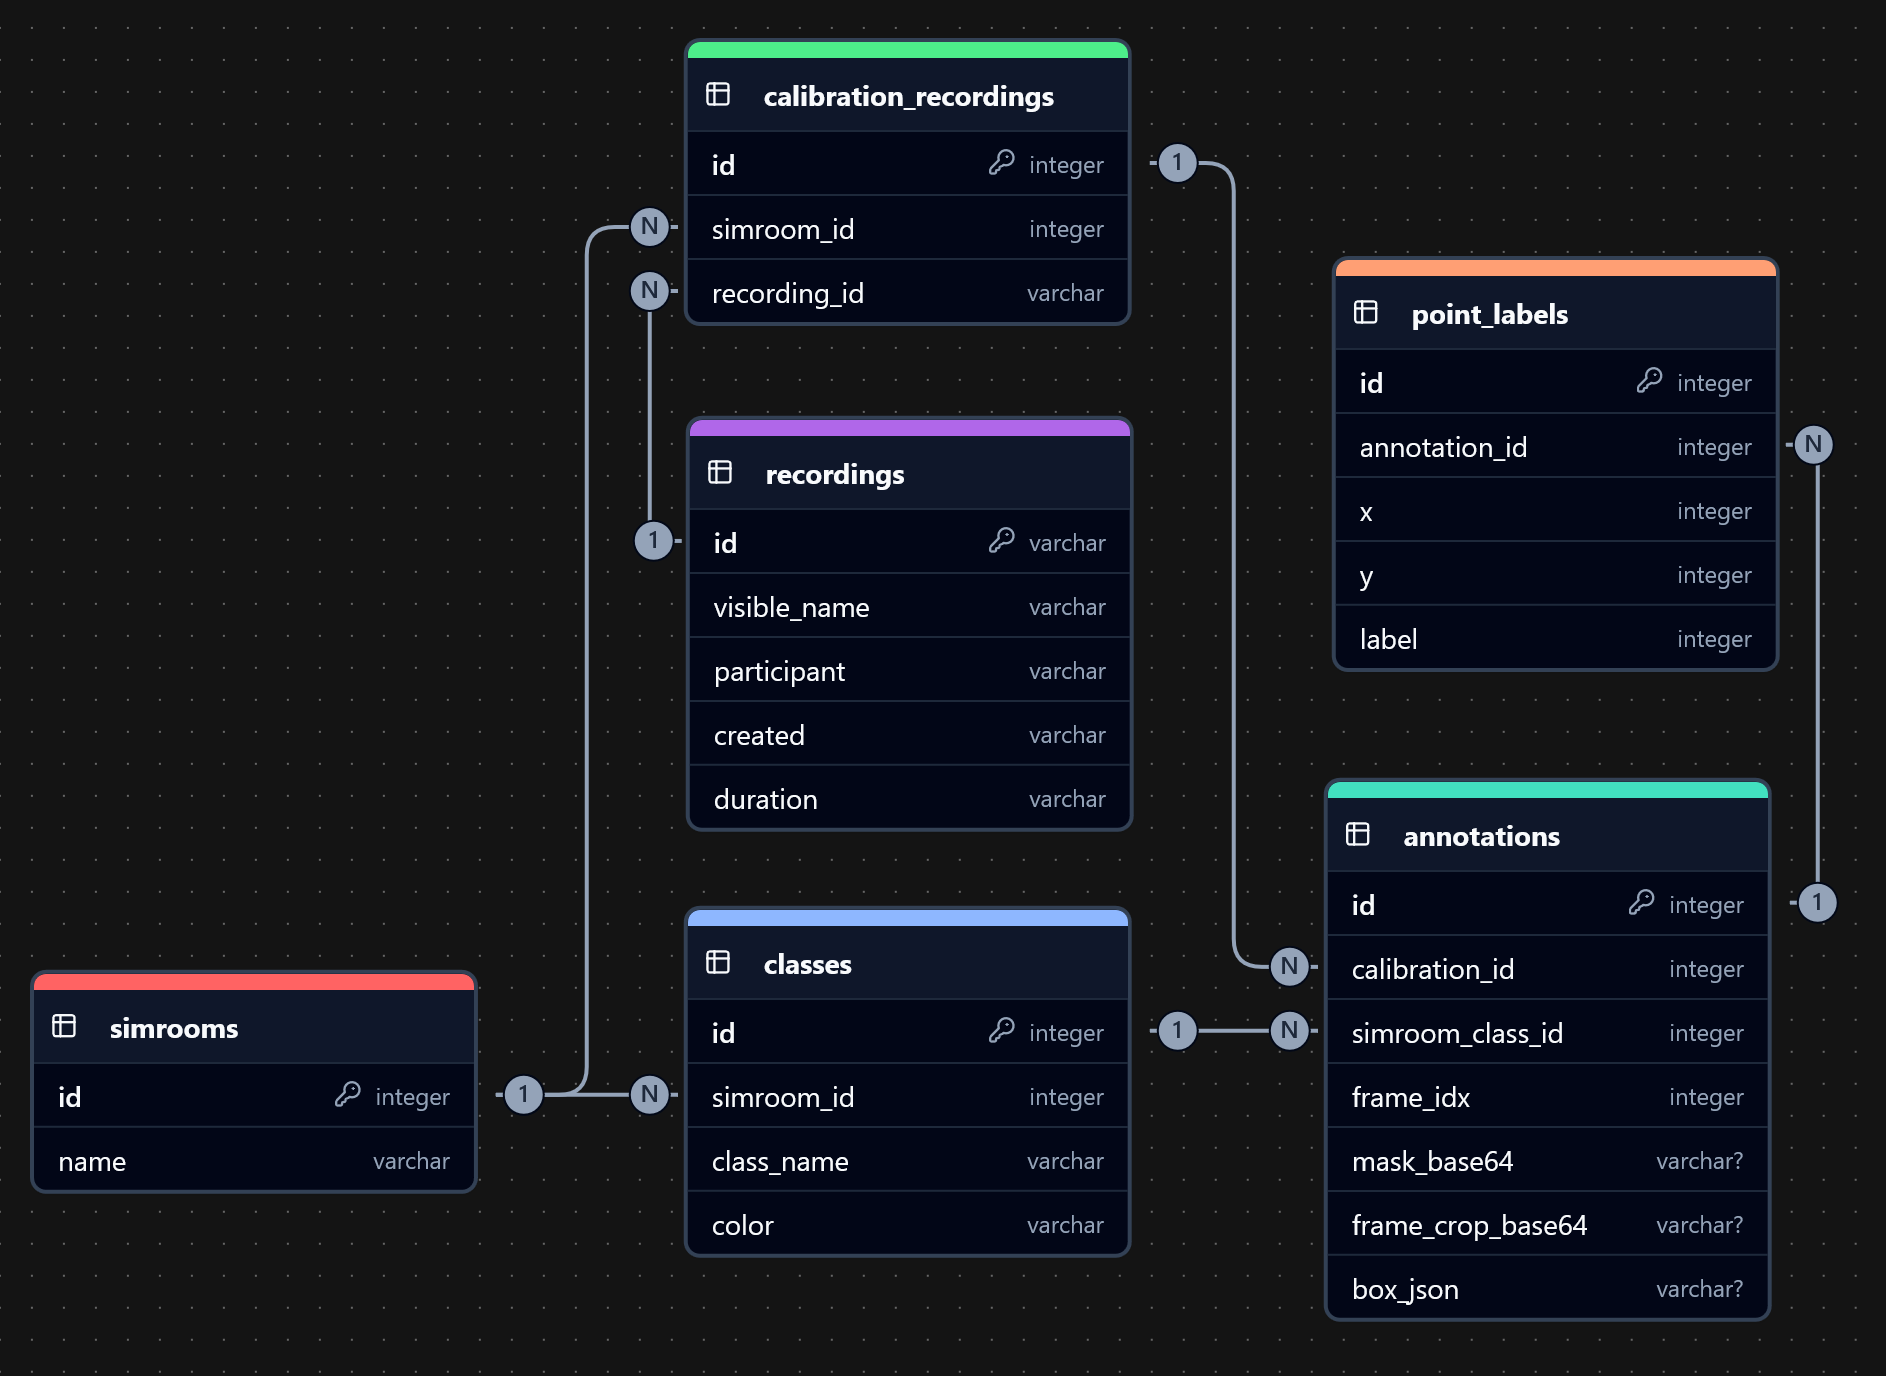
\includegraphics[width=0.8\textwidth]{erd.png}
  \caption[]{\label{fig:erd} Entity-Relationship Diagram (ERD) van de applicatie. De verschillende entiteiten en hun onderlinge relaties worden weergegeven: simulatieruimten, objecten (classes), opnames, kalibratie-opnames, annotaties, en point-labels. }
\end{figure}

\begin{itemize}
  \item \textbf{simrooms} zijn de verschillende omgevingen waarin de opnames worden gemaakt. 
  Elke simulatieomgeving heeft een naam en kan meerdere objecten bevatten.
  \item \textbf{classes} zijn de verschillende objecten die in de simulatieomgeving aanwezig zijn. 
  Elk object heeft een naam, een kleur, en kan meerdere annotaties bevatten.
  \item \textbf{recordings} zijn de video-opnames die gemaakt worden met de eyetracker. 
  Elke opname heeft een naam, een datum, en een duur. 
  Een opname kan ook dienen als kalibratie-opname voor meerdere simulatieruimten. 
  Opnames hebben ook een pad naar hun video- en blikdata bestand. 
  Deze paden worden niet opgeslagen in de database, maar worden gegenereerd op basis van het \texttt{id} van de opname. 
  \item \textbf{calibration\_recordings} zijn louter een referentie naar de opname die als kalibratie-opname wordt gebruikt 
  voor de simulatieomgeving. Ze kunnen meerdere annotaties bevatten.
  \item \textbf{annotations} worden gemaakt in de labeling-tool en hebben een \texttt{class}, een \texttt{frame index}, 
  een base64-gecodeerde afbeelding van het masker evenals van de regio in de originele frame. Het bevat eveneens een bounding box. Zowel het base64-gecodeerde 
  masker en de bounding-box worden getoond in de labeler bovenop de originele frame. De bounding-box is de rechthoek die de regio van de 
  annotatie omsluit, met het json formaat: \texttt{[x1, y1, x2, y2]}. Hier zijn \texttt{x1} en \texttt{y1} de coördinaten van de 
  linkerbovenhoek van de rechthoek, en \texttt{x2} en \texttt{y2} de coördinaten van de rechteronderhoek. 
  Tenslotte wordt ook een `crop' van de originele frame opgeslagen, dat enkel de regio van de annotatie bevat. 
  Dit is een afbeelding van dezelfde grootte als het masker, en wordt gebruikt om de annotatie te tonen in de annotatielijst onderaan de labeler.
  \item \textbf{point\_labels} zijn de individuele punten die aan een annotatie worden toegekend. Elk point-label heeft een x- en y-coördinaat, en een label dat aangeeft of het punt binnen (1) of buiten (0) de annotatie ligt.
\end{itemize}

Merk op dat de geautomatiseerde tracking-resultaten niet in de database worden opgeslagen, maar enkel de manuele annotaties.
Dit is omdat tracking grote hoeveelheden data generereert die op een optimale manier moeten worden opgeslagen.
De tracking-resultaten worden opgeslagen in een aparte map, onderverdeeld per kalibratie-opname en per klasse.
Elke file bevat de tracking-resultaten van één object in één kalibratie-opname, met als naam het frame index.
Ze worden opgeslagen in \texttt{.npz}-bestanden, die een gecomprimeerd formaat zijn voor numpy arrays.
Ze bevatten de volgende data:
\begin{itemize}
  \item \texttt{mask}: de gecomprimeerde versie van het masker dat werd gegenereerd door het segmentatie-algoritme.
  \item \texttt{bbox} \texttt{[x1, y1, x2, y2]}: de coördinaten van de bounding-box die het object omsluit.
  \item \texttt{roi} (Region of Interest): de regio van de originele frame die overeenkomt met het masker.
  \item \texttt{class\_id}: de id van de klasse waartoe het object behoort. 
  Zo kan andere informatie over het object---zoals de naam en de kleur---worden opgehaald uit de database.
  \item \texttt{frame\_index}: de index van het frame waarin het object werd getracked.
\end{itemize}

\section{Installatie en Configuratie}

TODO
% TODO: afwerken

\section{Gekende Problemen en Beperkingen}

Hoewel de kernfunctionaliteit van de applicatie robuust is, zullen we het in deze sectie hebben 
over enkele gekende problemen en beperkingen die de gebruikerservaring kunnen beïnvloeden.

% TODO: afwerken

\paragraph{Importeren van Opnames}

\paragraph{Labeling Tool}

\subsection{}
